\mychapter{Sistema proposto}
\label{cap:sistema}
Existem diversos métodos consolidados para detecção e isolamento de falhas,
sendo alguns deles baseados em redundância física de componentes de hardware,
como sensores, atuadores e controladores. Entretanto, a duplicação de
componentes de hardware nem sempre é possível, uma vez que os custos
relacionados com a adição de novos componentes podem elevar o orçamento
demasiadamente.

Devido a esse elevado custo, existe uma fronteira clara e inerente à aplicação
de técnicas de tolerância a falhas. A escolha adequada dos dispositivos físicos
e dos {\it softwares} devem levar em consideração as exigências específicas de
cada sistema, de tal maneira que se possa contornar o custo associado ao emprego
dessas técnicas \cite{weber:2002}.

Assim sendo, a primeira parte deste capítulo descreverá em detalhes o modelo de
estudo de caso escolhido, mostrando suas características e limitações.  Em
seguida a atenção será voltada para as estruturas neurais de identificação do
modelo e de detecção das falhas, mostrando ao final como serão realizadas as
simulações.

% ------------------------------------------------------------------------------
\section{Estudo de caso}
Ao final do Cap. \ref{cap:introducao}, propôs-se que seria desenvolvido um
sistema para realizar a DDF em um processo dinâmico. Para que isso fosse
possível seriam utilizadas estruturas neurais que fariam uso de determinados
valores, obtidos a partir das medições realizadas no processo e de seu histórico
de funcionamento.

O processo em questão, é formado por um sistema de tanques acoplados
desenvolvidos pela Quanser\reg, representado esquematicamente na Fig.
\ref{fig:tanques}.

\begin{figure}[htb]
\centering
    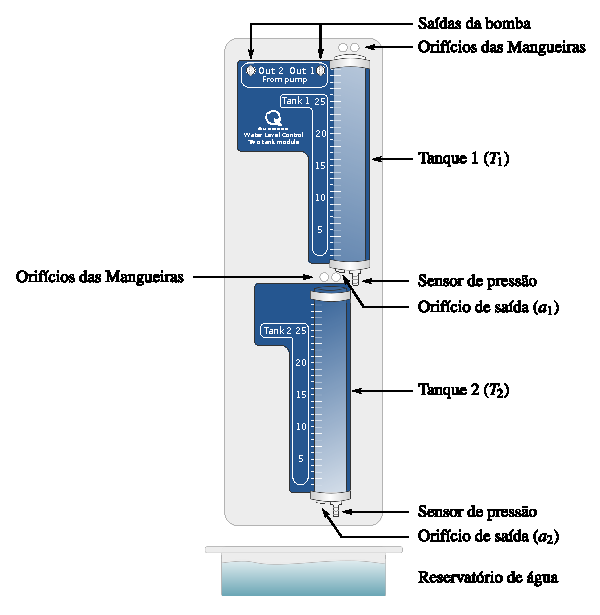
\includegraphics[width=0.7\textwidth]{imgs/sistema/eps/tanques}
    \caption{Sistema de tanques acoplados da Quanser\reg.}
    \label{fig:tanques}
\end{figure}

O sistema original consiste de uma bomba de água de corrente contínua e dois
tanques acoplados. A alimentação de água pela bomba se dá de forma vertical
através de dois orifícios com conectores normalmente fechados, de diferentes
diâmetros, denominados {\it Out 1} e {\it Out 2}. Para facilitar o entendimento
e evitar confusões com relação aos orifícios de saída dos tanques ($a_1$ e
$a_2$), esses orifícios serão tratados como orifícios de entrada.

\Glossary{$a_i$}{Orifício de saída $i$}

Os tanques ($T_1$ e $T_2$) são montados na parte frontal do suporte de base e
posicionados de tal forma que a água flui do tanque superior ($T_1$) para o
tanque inferior ($T_2$) através do orifício $a_1$, e do tanque inferior para o
reservatório através do orifício $a_2$. As vazões de saída dos tanques variam de
acordo com a mudança desses orifícios, disponibilizados em três diâmetros
diferentes pelo fabricante.

\Glossary{$T_1$}{Tanque superior}
\Glossary{$T_2$}{Tanque inferior}

Além dos diferentes orifícios de saída, o fabricante também disponibiliza um
conjunto de mangueiras, permitindo a utilização dos dois orifícios de entrada e
o bombeio de água para os dois tanques simultaneamente. As dimensões de cada um
dos orifícios e os demais parâmetros do sistema podem ser visualizados na Tab.
\ref{tab:dimensoes}.

\begin{table}[!htb]
\small
\centering
\caption{Dimensões e parâmetros do sistema de tanques.}
\label{tab:dimensoes}
\vspace{0.25cm}
\begin{tabular}{|l|c|c|c|}
\hline
{\bf Nome} & {\bf Símbolo} & {\bf Valor} & {\bf Unidade}\\
\hline
\hline
\multicolumn{4}{|l|}{{\bf Bomba}}\\
\hline
Constante de fluxo & $K_m$ & 4,6 & (cm${}^3$/s)/V\\
\hline
Limites de Tensão & $V_{p_{\text{\tiny MAX/MIN}}}$ & $\pm 15$ & Volts\\
\hline
Orifício de entrada 1 & {\it Out 1} & 0,635 & cm\\
\hline
Orifício de entrada 2 & {\it Out 2} & 0,4763 & cm\\
\hline
\multicolumn{4}{|l|}{{\bf Tanque 1/Tanque 2}}\\
\hline
Altura & $H_1$/$H_2$ & 30 & cm\\
\hline
Diâmetro interno & -- & 4,445 & cm\\
\hline
Área de secção transversal & $A_1$/$A_2$ & 15,517916547 & cm${}^2$\\
\hline
Sensibilidade do sensor & -- & 5 & cm/V \\
\hline
\multicolumn{4}{|l|}{{\bf Orifícios de saída -- Diâmetros}}\\
\hline
Orifício pequeno & $a_{i_{\text{\tiny PEQ}}}$ & 0,3175 & cm\\
\hline
Orifício médio & $a_{i_{\text{\tiny MED}}}$ & 0,47625 & cm\\
\hline
Orifício grande & $a_{i_{\text{\tiny GDE}}}$ & 0,555625 & cm\\
\hline
\multicolumn{4}{|l|}{{\bf Orifícios de saída -- Áreas}}\\
\hline
Orifício pequeno & $a_{i_{\text{\tiny PEQ}}}$ & 0,079173044 & cm${}^2$\\
\hline
Orifício médio & $a_{i_{\text{\tiny MED}}}$ & 0,178139348 & cm${}^2$\\
\hline
Orifício grande & $a_{i_{\text{\tiny GDE}}}$ & 0,242467446 & cm${}^2$\\
\hline
\multicolumn{4}{|l|}{{\bf Sensores}}\\
\hline
{\it Range} de pressão & -- & 0 - 1 & PSI\\
\hline
{\it Range} de nível & -- & 0 - 30 & cm\\
\hline
Constante de sensibilidade & $K_s$ & $6,25\times$ & cm/V\\
\hline
\end{tabular}
\end{table}

Dentre as várias combinações possíveis obtidas a partir da mudança dos orifícios
de entrada e saída, as três configurações sugeridas pelo manual do fabricante
encontram-se representadas na Fig. \ref{fig:config_fab}. Cada uma dessas
configurações modifica a dinâmica do processo, permitindo que sejam projetados e
analisados diferentes tipos de controladores.

\begin{figure}[!htb]
\centering
\subfigure[Configuração 1.]
{
    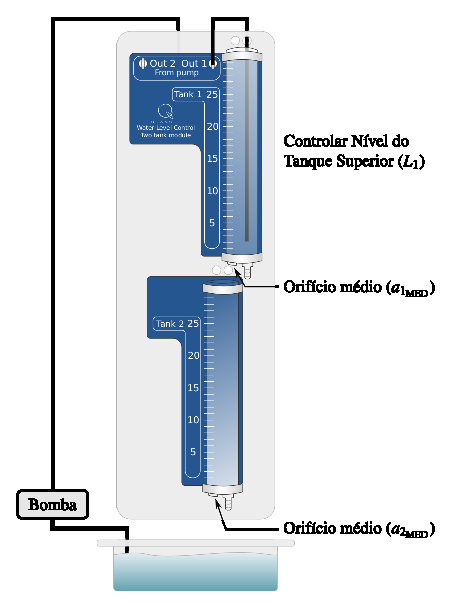
\includegraphics[width=0.31\textwidth]{imgs/sistema/eps/config_fab_1}
    \label{fig:config_fab_1}
}
\subfigure[Configuração 2.]
{
    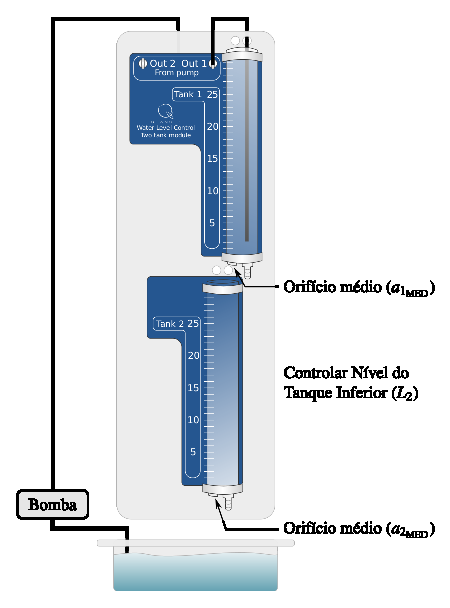
\includegraphics[width=0.31\textwidth]{imgs/sistema/eps/config_fab_2}
    \label{fig:config_fab_2}
}
\subfigure[Configuração 3.]
{
    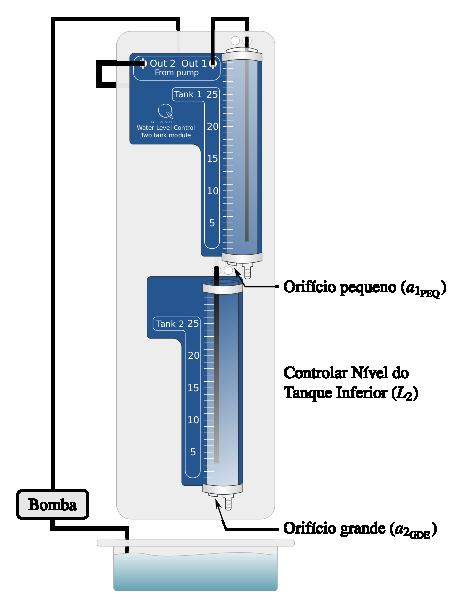
\includegraphics[width=0.31\textwidth]{imgs/sistema/eps/config_fab_3}
    \label{fig:config_fab_3}
}
\caption{Configurações sugeridas pelo fabricante.}
\label{fig:config_fab}
\end{figure}

Na primeira configuração deseja-se controlar o nível de $T_1$ ($L_1$) através de
uma alimentação direta, não fazendo uso do segundo tanque. Na segunda
configuração deseja-se controlar o nível de $T_2$ ($L_2$) a partir de uma
alimentação indireta em $T_1$. Assim, $T_2$ é alimentado a partir da água que
escoa de $T_1$ pelo orifício $a_1$. Por fim, na terceira configuração, deseja-se
controlar o nível de $T_2$ a partir de uma alimentação indireta em $T_1$ e da
alimentação direta de $T_2$. Para isso, faz-se uso dos dois orifícios de
entrada.

\Glossary{$L_1$}{Nível do tanque superior}
\Glossary{$L_2$}{Nível do tanque inferior}

Em todos os casos pode-se perceber que o sistema se comporta como um sistema de
uma única entrada, que é a tensão de alimentação da bomba, e uma única saída
({\it Single Input and Single Output} -- SISO), que pode ser $L_1$ ou $L_2$,
dependendo da configuração.

\Glossary{SISO}{{\it Single Input and Single Output}}

Além dessas observações, deve-se destacar ainda que a planta em questão faz
parte de um modelo desenvolvido para fins acadêmicos e que, por esse motivo,
existem algumas restrições quanto as interfaces e aos padrões de comunicação.

% ------------------------------------------------------------------------------
\subsection{Modelo matemático}

Como os dois tanques possuem mesma área de secção transversal ($A_1 = A_2$),
suas dinâmicas serão semelhantes. Entretanto, encontrar um modelo matemático que
descreva adequadamente a dinâmica desses tanques não é algo tão simples, visto
que as equações gerais de movimento e energia que descrevem o escoamento de
fluidos são bastante complicadas \cite{dorf:2009}.

Assim sendo, é preciso que sejam feitas algumas hipóteses fundamentais.
Admite-se que a água no tanque é incompressível e que o escoamento é
não-viscoso, não-rotacional e regular. Cada uma dessas características serão
descritas a seguir baseadas na argumentação exposta em \citeasnoun{dorf:2009}.

Diz-se que um fluido é incompressível quando este possui uma massa específica
constante. Entretanto, sabe-se que todo fluido é compressível em certo grau, e
que, o fator de compressibilidade $k$ é uma medida de tal característica.
Quanto menor o valor de $k$, menor é a compressibilidade indicada para aquele
fluido. O ar, que é um fluido compressível, possui um fator de compressibilidade
$k_{\text{ar}} = 0,98\ \text{m}^2/\text{N}$, enquanto que a água tem um fator de
compressibilidade de $k_{\tiny \text{\tiny H}_2\text{\tiny O}} = 4,9 \times
10^{-10}\ \text{m}^2/\text{N} = 50 \times 10^{-6}\ \text{atm}^{-1}$. Em outras
palavras, um dado volume de água diminui em 50 milionésimos de seu volume
original para um aumento de uma atmosfera de pressão. Desse modo, a hipótese de
que a água é incompressível é valida para o sistema em questão.

Já a viscosidade de um fluido é dada pelo seu coeficiente de viscosidade $\mu\
(\text{N}\cdotp \text{s}/\text{m}^2)$. Quanto maior esse coeficiente, mais
viscoso é o fluido. Como exemplo, o coeficiente de viscosidade em condições
normais à 20\textdegree C para o ar é $\mu_{\text{ar}} = 0,178 \times 10^{-4}\
\text{N}\cdotp \text{s}/\text{m}^2$ enquanto que para a água
$\mu_{\tiny \text{\tiny H}_2\text{\tiny O}} = 1,054 \times 10^{-3}\
\text{N}\cdotp \text{s}/\text{m}^2$. Assim, a água é cerca de 60 vezes mais
viscosa que o ar.  Vale salientar que a viscosidade depende principalmente da
temperatura e não da pressão. Para efeitos de comparação, a água à 0\textdegree
C é 2 vezes mais viscosa que a água à 20\textdegree C. Com fluidos de baixa
viscosidade como o ar e a água, os efeitos do atrito são importantes apenas nas
camadas de fronteira e em uma fina camada adjacente à parede do reservatório e
da tubulação de saída.  Assim, pode-se desprezar a viscosidade no
desenvolvimento do modelo.

\Glossary{$\mu_{\text{ar}}$}{Coeficiente de viscosidade do ar}
\Glossary{$\mu_{\tiny \text{\tiny H}_2\text{\tiny O}}$}
         {Coeficiente de viscosidade da água}

Se cada elemento do fluido em cada ponto do escoamento não tem velocidade
angular com relação a esse ponto, o fluxo é denominado não-rotacional. Admita
que a água no tanque é não-rotacional. Logo, para um fluido não-viscoso, um
fluxo inicialmente não-rotacional permanece não-rotacional.

Por fim, o fluxo de água é dito regular se sua velocidade em cada ponto é
constante com o tempo. Isso não implica necessariamente que a velocidade seja a
mesma em cada ponto, mas sim que em qualquer ponto a velocidade não mude com o
tempo. Condições de regime regular podem ser atingidas em velocidades baixas do
fluido. Admita então que há condições de fluxo regular. Observa-se entretanto
que se a área de abertura de saída fosse muito grande, o fluxo através do
reservatório não seria lento o suficiente para o estabelecimento das
condições de regime regular o que faria com que o modelo não conseguisse
predizer o fluxo do fluido de maneira exata.

Tendo esclarecido essas condições, para se obter o modelo matemático do fluido
dentro do reservatório emprega-se os princípios básicos da ciência e da
engenharia, como o princípio da conservação da massa. Assim, a massa de água em
qualquer instante de tempo é dada pela Eq. \ref{eq:conserv}.

\begin{equation}\label{eq:conserv}
m = \rhoagua\ AL
\end{equation}

\noindent em que $\rho_{\tiny \text{\tiny H}_2\text{\tiny O}}$ é a massa
específica da água, $A$ a área de secção transversal do reservatório e $L$ o
nível de água no reservatório. Tomando a derivada temporal de $m$ na Eq.
\ref{eq:conserv}, tem-se:

\begin{equation}
\dot{m} = \rhoagua\ A\dot{L}
\end{equation}

\noindent na qual utilizou-se o fato do fluido ser incompressível (ou seja,
$\dot{\rho} = 0$). Como a área de secção transversal não varia com o tempo, a
mudança de massa no reservatório é igual a massa que entra menos a massa que
deixa o tanque, logo:
 
\begin{equation}\label{eq:mudanca_massa}
\dot{m} = \rhoagua\ A\dot{L} = 
            Q_{\text{\tiny IN}} - 
\underbrace{\rhoagua\ a\upsilon_{\text{\tiny OUT}}}_
           {Q_{\text{\tiny OUT}}}
\end{equation}

\noindent em que $Q_{\text{\tiny IN}}$ é a vazão de entrada de massa em regime
permanente, $a$ é a área do orifício de saída e $\upsilon_{\text{\tiny OUT}}$ é
a velocidade de saída do fluido, que é uma função da altura da água. Da equação
de Bernoulli \cite{houghton:2002}, tem-se:

\begin{equation}
P_{\text{\tiny IN}} + 
\frac{1}{2}\rhoagua\ {\upsilon_{\text{\tiny IN}}}^2 +
\rhoagua\ gL
=
\frac{1}{2}\rhoagua\ {\upsilon_{\text{\tiny OUT}}}^2 +
P_{\text{\tiny OUT}}
\end{equation}

\noindent em que $\upsilon_{\text{\tiny IN}}$ é a velocidade da água na entrada
do reservatório e $P_{\text{\tiny IN}}$ e $P_{\text{\tiny OUT}}$ são as pressões
na entrada e na saída, respectivamente. Mas $P_{\text{\tiny IN}}$ e
$P_{\text{\tiny OUT}}$ são iguais à pressão atmosférica e a área de $a$ é
suficientemente pequena ($a \approx A/85$, considerando o orifício de saída
médio) para que a água escoe vagarosamente e a velocidade $\upsilon_{\text{\tiny
IN}}$ seja desprezível. Assim, a equação de Bernoulli fica reduzida a:

\begin{equation}\label{eq:bernoulli_red}
\upsilon_{\text{\tiny OUT}} = \sqrt{2gL}
\end{equation}

Além disso, segundo \citeasnoun{apkarian:1999}, a vazão de entrada
$Q_{\text{\tiny IN}}$ depende apenas da constante da bomba e da tensão à ela
aplicada, podendo ser positiva, quando a água é sugada do reservatório e
injetada no tanque, ou negativa quando a água é sugada do tanque e devolvida ao
reservatório. Assim:

\begin{equation}\label{eq:vazao_ent}
Q_{\text{\tiny IN}} = K_mV_p
\end{equation}

Substituindo então as Eqs. \ref{eq:bernoulli_red} e \ref{eq:vazao_ent} na Eq.
\ref{eq:mudanca_massa} e resolvendo para $\dot{L}$, tem-se:

\begin{equation}\label{eq:l_ponto}
\dot{L} = -\left[\frac{a}{A}\sqrt{2g}\right]\sqrt{L} + 
          \frac{1}{\rhoagua\ A}K_mV_p
\end{equation}

Considerando que a massa específica da água é $\rhoagua \approx 1,0$ à
20\textdegree C, então a Eq. \ref{eq:l_ponto} passa a ser:

\begin{equation}\label{eq:l_ponto_final}
\dot{L} = -\left[\frac{a}{A}\sqrt{2g}\right]\sqrt{L} + 
          \frac{K_m}{A}V_p
\end{equation}

Assim, as duas únicas variáveis do modelo serão o nível $L$ do tanque e a tensão
$V_p$ aplicada à bomba. Perceba que essa é uma equação diferencial ordinária
não-linear.

% ------------------------------------------------------------------------------
\subsection{Modificações do modelo}
Observa-se que Eq. \ref{eq:l_ponto_final} representa adequadamente a dinâmica do
tanque superior, contudo, a dinâmica do tanque inferior age um pouco diferente.
Em primeiro lugar, dependendo da configuração escolhida $T_2$ poderá ou não
receber uma alimentação direta. Considerando, por exemplo, a primeira
configuração sugerida pelo manual do fabricante, mostrada na Fig.
\ref{fig:config_fab_1}, a dinâmica de $T_2$ irá depender apenas da vazão de água
que escoa de $T_1$ e da vazão de água que retorna ao reservatório. Assim sendo,
a dinâmica dos dois tanques pode ser representada pelas Eqs.
\ref{eq:l1_ponto_tmp} e \ref{eq:l2_ponto_tmp}:

\begin{eqnarray}
\dot{L_1} & = & \frac{K_m}{A}V_p -
                \left[\frac{a_1}{A}\sqrt{2g}\right]\sqrt{L_1}
                \label{eq:l1_ponto_tmp}\\
\dot{L_2} & = & \left[\frac{a_1}{A}\sqrt{2g}\right]\sqrt{L_1} -
                \left[\frac{a_2}{A}\sqrt{2g}\right]\sqrt{L_2}
                \label{eq:l2_ponto_tmp}
\end{eqnarray}

\noindent em que $a_1$ representa o orifício de saída de $T_1$, $a_2$ o orifício
de saída de $T_2$, $L_1$ o nível de água em $T_1$ e $L_2$ o nível e água em
$T_2$. Perceba que não há necessidade em se discriminar a área de secção
transversão através de um subíndice, pois $A_1 = A_2 = A$.

Com o intuito de deixar o sistema proposto com um caráter mais genérico e
possibilitar que sejam realizados novos estudos relacionados com o tema de
tolerância à falhas, optou-se por modificar o sistema de tanques original
introduzindo uma outra bomba com as mesmas características da primeira. Dessa
forma, pôde-se obter novas configurações, dentre as quais destacam-se aquelas
expostas pela Fig. \ref{fig:novas_config}.

\begin{figure}[htb]
\centering
\subfigure[Nova configuração 1.]
{
    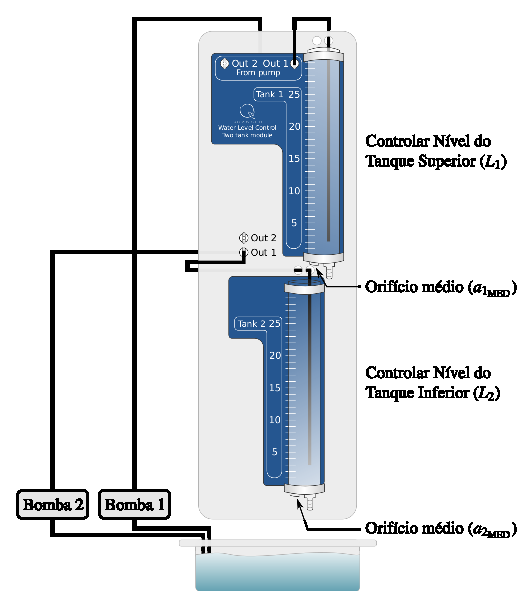
\includegraphics[width=0.45\textwidth]{imgs/sistema/eps/nova_config_1}
    \label{fig:nova_config_1}
}
\subfigure[Nova configuração 2.]
{
    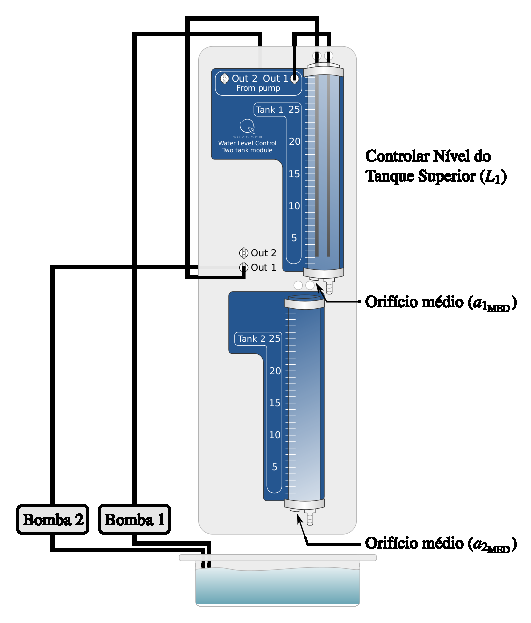
\includegraphics[width=0.45\textwidth]{imgs/sistema/eps/nova_config_2}
    \label{fig:nova_config_2}
}
\caption{Novas configurações sugeridas após a modificação do modelo.}
\label{fig:novas_config}
\end{figure}

Na configuração exposta pela Fig. \ref{fig:nova_config_1}, pode-se controlar o
nível dos dois tanques de maneira individual através das duas bombas de água.
\begin{comment}
Para isso, pode-se implementar dois controladores cada um com sua referência e a
leitura do respectivo sensor ou um único controlador que receberá as duas
referências e as leituras dos dois sensores.
\end{comment}
Já na configuração exposta pela Fig. \ref{fig:nova_config_2}, a segunda bomba
está sendo utilizada para garantir que o processo continue funcionando
normalmente quando a primeira bomba vier a falhar. Ou seja, possui-se dois
atuadores com um deles em {\it standby}. Ademais, é válido ressaltar que essa
última configuração pode ser facilmente adaptada para qualquer uma das três
anteriores sugeridas pelo fabricante.

É evidente que, no caso da Fig. \ref{fig:nova_config_1}, o sistema deixa de ser
SISO e passa a ser MIMO. Por esse motivo, esse sistema será o utilizado como
modelo de estudo de caso no trabalho. A única modificação existente nas equações
que regem a dinâmica do modelo é a introdução de uma nova variável na equação do
segundo tanque, em virtude da adição da segunda bomba. Assim, as equações finais
do modelo de estudo de caso serão:

\begin{eqnarray}
\dot{L_1} & = & \frac{K_m}{A}V_{p_{\tiny 1}} -
                \left[\frac{a_1}{A}\sqrt{2g}\right]\sqrt{L_1}
                \label{eq:l1_ponto}\\
\dot{L_2} & = & \frac{K_m}{A}V_{p_{\tiny 2}} +
                \left[\frac{a_1}{A}\sqrt{2g}\right]\sqrt{L_1} -
                \left[\frac{a_2}{A}\sqrt{2g}\right]\sqrt{L_2}
                \label{eq:l2_ponto}
\end{eqnarray}

\noindent em que $V_{p_{\tiny 1}}$ se refere à tensão aplicada na Bomba 1
($B_1$) e $V_{p_{\tiny 2}}$ à tensão aplicada na Bomba 2 ($B_2$).

\Glossary{$B_i$}{Bomba $i$}

% ------------------------------------------------------------------------------
\section{Limitações do processo}\label{sec:limitacoes}
Conforme dito anteriormente, a planta do estudo de caso foi desenvolvida para
fins acadêmicos e possui algumas limitações com relação as interfaces e aos
padrões de comunicação. Por causa dessas limitações a planta é normalmente
controlada por um sistema desenvolvido computacionalmente em que a comunicação
se dá através de um barramento ISA ({\it Industry Standard Architecture}). Tal
sistema deve calcular as ações de controle proporcional, integral e derivativa e
produzir um sinal de controle em Volts que será enviado aos atuadores.

\Glossary{ISA}{{\it Industry Standard Architecture}}

Entretanto, devido aos baixos níveis de tensão intrínsecos à esse tipo de
barramento, faz-se necessário utilizar um amplificador, também fornecido pela
Quanser\reg, cujo fator de amplificação é de cinco vezes. Assim, para que a
bomba não venha a queimar, os sistemas de controle devem implementar uma rotina
de segurança que garanta que o sinal de controle não supere os limites de $\pm
3$ Volts. A representação esquemática do funcionamento do sistema como um todo
está representada na Fig. \ref{fig:func_sistema}.

\begin{figure}[htb]
\centering
    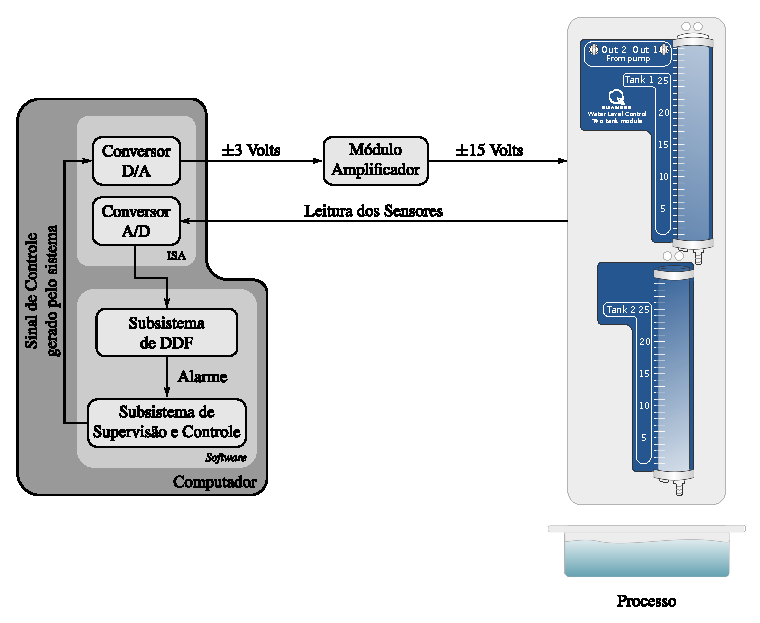
\includegraphics[width=0.8\textwidth]{imgs/sistema/eps/func_sistema}
    \caption{Diagrama esquemático de funcionamento do sistema proposto.}
    \label{fig:func_sistema}
\end{figure}

A partir dessa representação esquemática, percebe-se facilmente que as únicas
variáveis disponíveis são os níveis dos tanques ($L_1$ e $L_2$) e as tensões das
bombas ($V_{p_{\tiny 1}}$ e $V_{p_{\tiny 2}}$).

Além das limitações físicas relacionadas aos sinais enviados ou recebidos pelo
processo, destaca-se ainda o fato de se tratar de uma planta real em que todos
os dispositivos físicos e mecânicos estão sujeitos a deteriorações relacionadas
ao tempo de uso. Assim sendo, não se considera uma boa prática estimular ou
induzir falhas no sistema real. Logo, todas as falhas a serem analisadas serão
induzidas através do modelo matemático simulado em um sistema computacional.

% ------------------------------------------------------------------------------
\section{Simulações do sistema e das falhas}
Considerando os fatores expostos ao final da seção \ref{sec:limitacoes}, o
sistema de tanques será simulado a partir das Eqs. \ref{eq:l1_ponto} e
\ref{eq:l2_ponto}, utilizando o método de Runge-Kutta de 4\textordfeminine\
ordem (RK4).

\Glossary{RK4}{Método de Runge-Kutta de 4\textordfeminine\ ordem}

De maneira resumida, pode-se dizer que o RK4 faz parte de uma família de métodos
interativos para a aproximação numérica de soluções de equações diferenciais
ordinárias. O funcionamento do método pode ser esclarecido conforme explicação a
seguir. 

Seja um problema de valor inicial dado por:

\begin{equation}\label{eq:}
y' = f(t,y) \qquad y(t_0) = y_0
\end{equation}

Então, o método RK4 para este problema é dado pelas seguintes equações:

\begin{eqnarray}
y_{n+1} & = & y_n + \frac{h}{6}\left(k_1 + 2k_2 + 2k_3 + k_4\right)\\
t_{n+1} & = & t_n + h
\end{eqnarray}

\noindent em que $y_{n+1}$ é a aproximação por RK4 de $y(t_{n + 1})$, e:

\begin{eqnarray}
k_1 & = & f\left(t_n,y_n\right)\\
k_2 & = & f\left(t_n+\frac{h}{2},y_n+\frac{h}{2}k_1\right)\\
k_3 & = & f\left(t_n+\frac{h}{2},y_n+\frac{h}{2}k_2\right)\\
k_4 & = & f\left(t_n+h,y_n+hk_3\right)
\end{eqnarray}

Assim, o próximo valor ($y_{n+1}$) é determinado a partir do valor atual ($y_n$)
somado com o produto do tamanho do intervalo ($h$) e uma inclinação estimada,
obtida a partir da média ponderada das inclinações $k_i$. Percebe-se ainda que a
média ponderada dá um maior peso para as inclinações no ponto médio.

\begin{comment}
\begin{itemize}
    \item $k_1$ é a inclinação no início do intervalo;
    \item $k_2$ é a inclinação no ponto médio do intervalo, usando $k_1$ para
determinar o valor de $y$ no ponto $t_n + h/2$ através do método de Euler;
    \item $k_3$ é novamente a inclinação no ponto médio do intervalo, usando
entretanto a inclinação $k_2$ para determinar o valor de $y$;
    \item $k_4$ é a inclinação no final do intervalo, com seu valor de $y$
determinado a partir de $k_3$.
\end{itemize}
\end{comment}

O método de RK4 permite que sejam determinados os valores de $L_1$ e $L_2$ para
cada instante da simulação e, consequentemente, que a dinâmica do processo seja
observada. As falhas induzidas no processo serão então computadas a partir de
alterações feitas sobre os valores de $L_1$ e $L_2$ obtidos. Dependendo do tipo
de falha, a alteração pode ocorrer antes, durante ou após a execução do método
de RK4.

% ------------------------------------------------------------------------------
\subsection{Falhas simuladas}
Assim como já foi visto, devido ao elevado grau de complexidade e à integração
inter processos, as falhas que antes poderiam ser detectadas através de medições
diretas de determinadas variáveis, passam a depender de um conjunto de variáveis
que atuam simultaneamente no sistema.  Ademais, as causas das falhas podem nem
sempre estar próximas dos locais em que foram identificadas.

Considerando tais aspectos, foram selecionadas somente algumas falhas dentre
aquelas que podem ocorrer no processo em estudo. Alguns exemplos de falhas desse
sistema podem ser observados na Tab. \ref{tab:selecao_falhas}. O agrupamento e a
classificação das falhas escolhidas se deu conforme Tabs.
\ref{tab:grupos_falhas} e \ref{tab:classificacao_falhas}.

\begin{table}[!htb]
\small
\centering
\caption{Exemplos de falhas que podem ocorrer no sistema de tanques.}
\label{tab:selecao_falhas}
\vspace{0.25cm}
\begin{tabular}{|c|c|c|}
\hline
{\bf Sensores} & {\bf Atuadores} & {\bf Estruturais}\\
\hline
\hline
Erro de leitura & Erro de escrita & Erro de transmissão\\
\hline
Descalibramento & Erro de leitura & Perda de comunicação\\
\hline
Sensibilidade à ruído & Sensibilidade à ruído & Sensibilidade à ruído\\
\hline
Queima do sensor & Queima do atuador & Queima do transmissor\\
\hline
-- & Atraso de transporte & Atraso de propagação\\
\hline
\end{tabular}
\end{table}

\begin{table}[!htb]
\small
\centering
\caption{Grupos de falhas.}
\label{tab:grupos_falhas}
\vspace{0.25cm}
\begin{tabular}{|c|c|c|}
\hline
{\bf Grupo} & {\bf Tipo de falha} & {\bf Sigla}\\
\hline
\hline
0 & Não há falhas & SF\\
\hline
1 & Falha do sensor & FSe\\
\hline
2 & Falha do atuador & FA\\
\hline
\multirow{2}{*}{3} & 
Falha estrutural ou & 
\multirow{2}{*}{FSi}\\
&
Falha do sistema & 
\\
\hline
\end{tabular}
\end{table}

\begin{table}[!htb]
\small
\centering
\caption{Classificação das falhas selecionadas.}
\label{tab:classificacao_falhas}
\vspace{0.25cm}
\begin{tabular}{|c|c|c|c|c|}
\hline
{\bf Grupo} & {\bf Classe} & {\bf Denominação} & {\bf Variante} & {\bf Sigla}\\
\hline
\hline
1 & 1 & Descalibramento & Ganho & FSeDG\\
\hline
1 & 1 & Descalibramento & Nível DC ({\it offset}) & FSeDO\\
\hline
1 & 2 & Sensibilidade & Ruído & FSeSR\\
\hline
1 & 3 & Queima & -- & FSeQ\\
\hline
\hline
2 & 1 & Descalibramento & Ganho & FADG\\
\hline
2 & 1 & Descalibramento & Nível DC ({\it offset}) & FADO\\
\hline
2 & 2 & Sensibilidade & Ruído & FASR\\
\hline
2 & 3 & Variação & Constante da bomba ($K_m$) & FAVK\\
\hline
2 & 4 & Queima & -- & FAQ\\
\hline
\hline
3 & 3 & Vazamento & Tanque & FSiVzT\\
\hline
3 & 2 & Variação & Orifício de saída & FSiVrOS\\
\hline
3 & 2 & Variação & Ganho do módulo de potência & FSiVrGMP\\
\hline
3 & 1 & Entupimento & Orifício de saída & FSiEOS\\
\hline
\end{tabular}
\end{table}

\Glossary{FSeDG}{Falha do Sensor por Descalibramento de Ganho}
\Glossary{FSeDO}{Falha do Sensor por Descalibramento de {\it Offset}}
\Glossary{FSeSR}{Falha do Sensor por Sensibilidade à Ruído}
\Glossary{FSeQ}{Falha do Sensor por Queima}
\Glossary{FADG}{Falha do Atuador por Descalibramento de Ganho}
\Glossary{FADO}{Falha do Atuador por Descalibramento de {\it Offset}}
\Glossary{FASR}{Falha do Atuador por Sensibilidade à Ruído}
\Glossary{FAVK}{Falha do Atuador por Variação da Constante da Bomba ($K_m$)}
\Glossary{FAQ}{Falha do Atuador por Queima}
\Glossary{FSiVzT}{Falha do Sistema por Vazamento do Tanque}
\Glossary{FSiVrOS}{Falha do Sistema por Variação do Orifício de Saída}
\Glossary{FSiVrGMP}{Falha do Sistema por Variação do Ganho do Módulo de 
                    Potência}
\Glossary{FSiEOS}{Falha do Sistema por Entupimento do Orifício de Saída}

As siglas expostas nessas tabelas foram introduzidas com o intuito de facilitar,
tanto o processo automático de treinamento e validação da estrutura neural,
quanto a referenciação textual.

As falhas expostas na Tab. \ref{tab:classificacao_falhas} são induzidas de
diferentes maneiras na simulação. Na FADG, por exemplo, o ganho do atuador é
alterado de 1,0 para qualquer outro valor a juízo do usuário, no momento em que é
realizada a leitura dos níveis. Já na FSiVzT, por questões de simplicidade,
adiciona-se um outro orifício ao lado do orifício de saída do tanque. Esse
orifício, de área arbitrária, terá a mesma dinâmica do orifício de saída do
tanque, exceto que para $T_1$ a água que por ele escoa não irá cair em $T_2$.

Para dar mais liberdade de configuração à simulação, foi desenvolvido um sistema
em C++, que implementa o método de RK4 e que possui a capacidade de configurar
todos os parâmetros referentes a cada uma dessas falhas a partir de um arquivo
de texto. Cada um dos parâmetros do arquivo de entrada deve ser especificado em
uma coluna e o número de linhas equivale ao número de amostras a serem
simuladas. O período de amostragem utilizado na simulação do sistema é de 100
(cem) milissegundos, o mesmo utilizado para o controle da planta real.

Além disso, o sistema implementa as rotinas de dois controladores que podem ser
configurados para operarem como controladores P, PI, PD, PID ou PI-D. Os ganhos
proporcionais, integrais e derivativos são introduzidos na interface do usuário.

Esse mesmo sistema pode ainda ser utilizado para operar com a planta real,
fazendo aquisições dos dados através da rede (local ou remota), utilizando {\it
sockets} TCP, se comunicando com um servidor implementado conforme mostrado em
\citeasnoun{oliveira:2008}. A configuração do endereço IP e da porta de
comunicação também é realizada a partir da interface do usuário. A Fig.
\ref{fig:captura} mostra uma captura de tela ({\it screenshot}) do sistema em
funcionamento.

\begin{figure}[htb]
\centering
    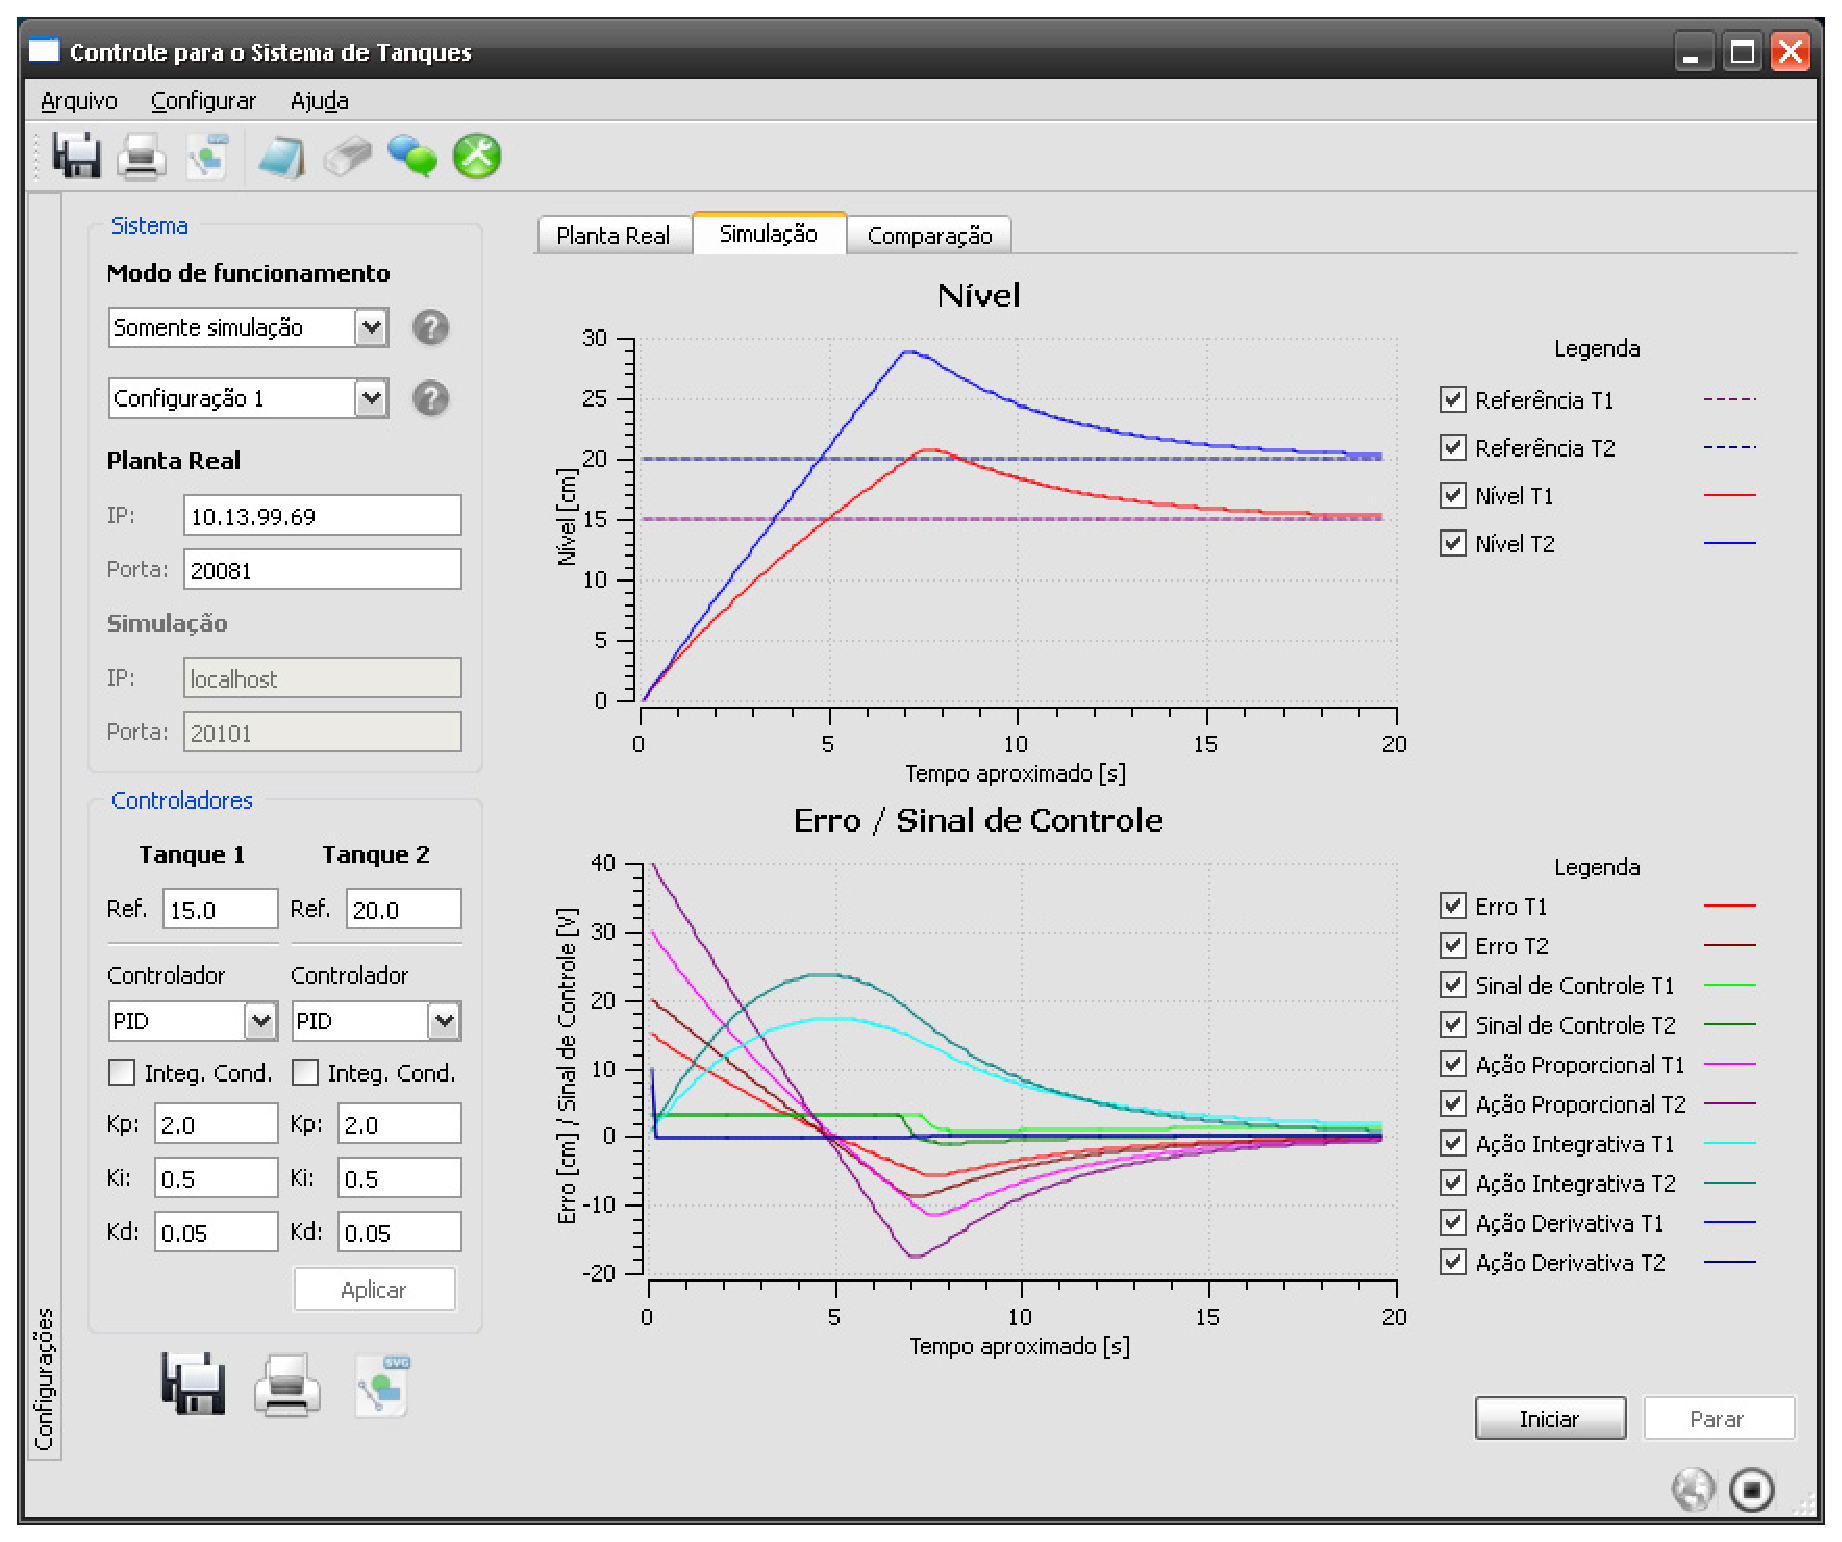
\includegraphics[width=0.75\textwidth]{imgs/sistema/eps/captura}
    \caption{Captura de tela do sistema em funcionamento.}
    \label{fig:captura}
\end{figure}

% ------------------------------------------------------------------------------
\section{Estruturas neurais escolhidas}
Tanto para a identificação do modelo quanto para a detecção e o diagnóstico das
falhas, deve-se ter bastante cuidado ao se escolher a estrutura e a arquitetura
das redes neurais. Em ambos os casos, uma escolha inadequada pode fazer com que
o sistema não se comporte de maneira adequada e não realize a função para o qual
foi designado. 

Assim sendo, para que fosse realizada uma análise comparativa, foram propostas
duas estruturas neurais para o processo de identificação do modelo e duas outras
estruturas para a detecção e o diagnóstico das falhas. Nos quatro casos foram
utilizados modelos NNARX com uma camada oculta com função de ativação sigmoidal
em que o número de regressores e o número de neurônios nessa camada foram
determinados a partir de testes, conforme mostrado no Cap. \ref{cap:resultados}.
Os detalhes relativos a cada uma dessas estruturas são esclarecidos nas próximas
seções.

% ------------------------------------------------------------------------------
\subsection{Propostas de identificação}
A primeira estrutura de identificação busca representar a dinâmica do sistema de
tanques através de uma única rede neural, a qual receberia como entrada os
valores passados dos níveis, $L_1(k-1)$ e $L_2(k-1)$, e os valores de tensão
aplicados, $V_{p_{\tiny 1}}(k-1)$ e $V_{p_{\tiny 2}}(k-1)$, gerando uma
estimativa dos níveis em sua saída, denominadas $\widehat{L_1}(k)$ e
$\widehat{L_2}(k)$.  A Fig. \ref{fig:ident_proposta_1} representa um diagrama
esquemático do funcionamento dessa primeira proposta.

\begin{figure}[htb]
\centering
    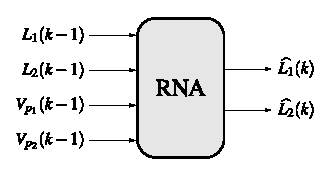
\includegraphics[width=0.38\textwidth]{imgs/sistema/eps/ident_proposta_1}
    \caption{Proposta de identificação global.}
    \label{fig:ident_proposta_1}
\end{figure}

Já a segunda estrutura de identificação leva em consideração que cada tanque
possui uma dinâmica diferente, tendo em vista que o $T_1$ age de maneira
independente, enquanto que a dinâmica de $T_2$ depende de $T_1$. Assim, optou-se
por utilizar duas redes neurais, como mostrado na Fig.
\ref{fig:ident_proposta_2}.

\begin{figure}[htb]
\centering
    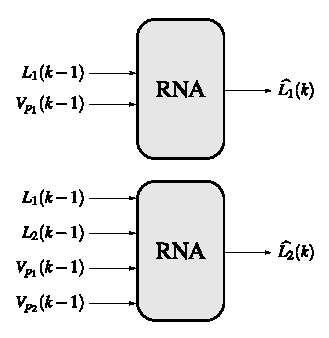
\includegraphics[width=0.38\textwidth]{imgs/sistema/eps/ident_proposta_2}
    \caption{Proposta de identificação individual.}
    \label{fig:ident_proposta_2}
\end{figure}

A primeira rede seria a responsável pela identificação de $T_1$, recebendo como
entrada o nível anterior, $L_1(k-1)$, e a tensão aplicada, $V_{p_{\tiny
1}}(k-1)$, gerando uma estimativa de $L_1$ em sua saída. Já a segunda rede seria
a responsável pela identificação da dinâmica de $T_2$ e receberia como entrada
as mesmas variáveis da primeira proposta, ou seja, $L_1(k-1)$, $L_2(k-1)$,
$V_{p_{\tiny 1}}(k-1)$ e $V_{p_{\tiny 2}}(k-1)$. A saída da segunda rede seria,
portanto, a estimativa do nível de $T_2$.

Independentemente da proposta, pode-se visualizar o sistema de identificação do
modelo como uma única estrutura neural (simples ou composta), que possui como
entrada os níveis anteriores e as tensões aplicadas, e que produz em sua saída
as estimativas dos níveis dos dois tanques. A Fig. \ref{fig:sist_ident} mostra
como o sistema de identificação pode ser visto.

\begin{figure}[!htb]
\centering
    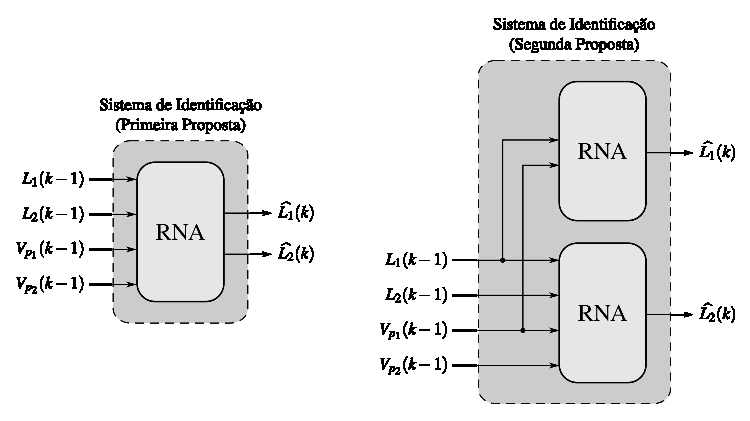
\includegraphics[width=0.875\textwidth]{imgs/sistema/eps/sist_ident}
    \caption{Visão geral do sistema de identificação.}
    \label{fig:sist_ident}
\end{figure}

% ------------------------------------------------------------------------------
\subsection{Propostas de detecção}
As estruturas neurais de DDF seguiram o mesmo raciocínio adotado para as
estruturas de identificação. No primeiro caso, buscou-se desenvolver uma única
rede neural que fosse capaz de detectar e identificar cada uma das falhas
listadas pela Tab. \ref{tab:classificacao_falhas}. Essa rede receberia como
entrada os mesmos sinais das redes de identificação e os resíduos $e_i$,
produzidos pela diferença dos níveis entre o modelo simulado ($L_i$) e o modelo
identificado ($\widehat{L_i}$). A saída da rede formaria uma palavra binária que
seria decodificada a partir de uma tabela previamente estabelecida. Nessa tabela
cada falha teria uma palavra binária correspondente.  A Fig.
\ref{fig:detec_prop_1} representa um diagrama esquemático dessa proposta.

\begin{figure}[!htb]
\centering
    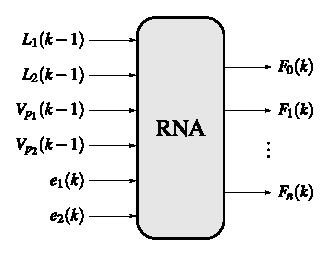
\includegraphics[width=0.37\textwidth]{imgs/sistema/eps/detec_prop_1}
    \caption{Proposta de detecção através de uma única rede neural.}
    \label{fig:detec_prop_1}
\end{figure}

Na segunda proposta, a estrutura de DDF seria composta por várias redes neurais,
em que cada uma destas estaria associada a uma única falha, formando um conjunto
de ``especialistas''. Não se trata, entretanto, de uma máquina de comitê de
especialistas, uma vez que não existe uma rede que realiza a tomada de decisões. 

Inicialmente, as entradas de cada uma das redes seriam as mesmas da primeira
proposta. As saídas, por sua vez, seriam compostas por uma palavra de apenas 2
bits, indicando se aquela falha estaria sendo detectada cada em $T_1$ em $T_2$
ou em $T_1$ e $T_2$ simultaneamente. A Fig. \ref{fig:detec_prop_2} representa um
diagrama esquemático dessa proposta.

\begin{figure}[!htb]
\centering
    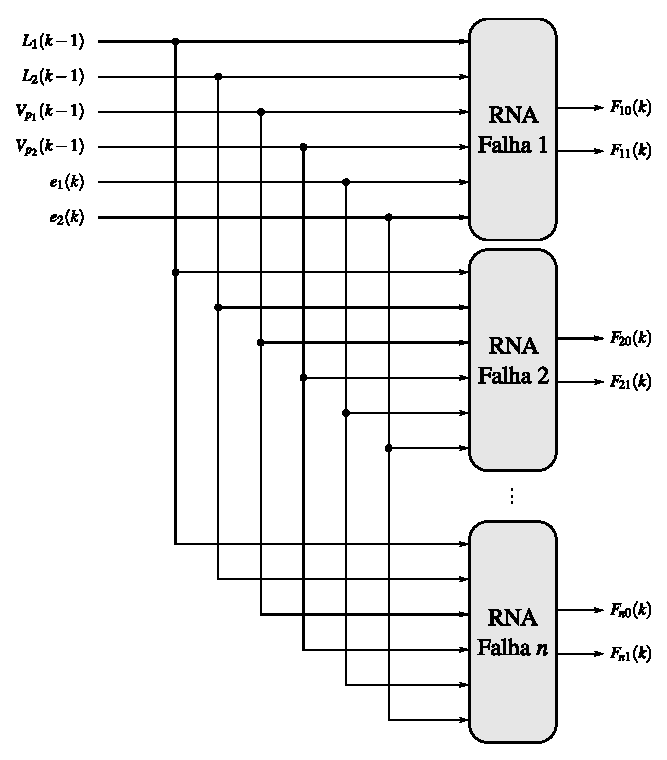
\includegraphics[width=0.725\textwidth]{imgs/sistema/eps/detec_prop_2}
    \caption{Proposta de detecção através de um conjunto de redes
             especialistas.}
    \label{fig:detec_prop_2}
\end{figure}

Existem diversas vantagens em se utilizar a segunda proposta ao invés da
primeira, como por exemplo, a de se utilizar entradas diferentes para cada uma
das redes especialistas. Essa situação poderia ocorrer se fosse percebido que
uma determinada entrada, ao ser adicionada, fizesse com que aquela falha fosse
detectada de maneira mais precisa ou mais rápida. Essa vantagem também é
percebida na situação inversa, em que uma determinada entrada pode estar sendo
indiferente com relação ao processo de detecção.

Modificar a estrutura das entradas na primeira proposta faria com que a rede
precisasse ser treinada novamente. Por se tratar, provavelmente, de uma
estrutura mais complexa, o treinamento poderia ter um grande custo relacionado
ao tempo e ao processamento. Já na segunda proposta apenas uma das redes seria
retreinada, o que iria reduzir esse custo de maneira considerável. Além disso,
se o treinamento fosse realizado em tempo real, não haveria necessidade de se
parar o sistema de detecção como um todo, mas somente uma parte deste. 

Uma outra vantagem estaria relacionada com o pós-processamento da informação. Ao
se utilizar a segunda proposta percebe-se que não é necessário realizar uma
decodificação da saída a cada vez que uma entrada é introduzida na rede.
Considerando que o tempo gasto para decodificar a palavra na saída da primeira
proposta, é diretamente proporcional ao tamanho da palavra e que este, por sua
vez, está diretamente relacionado com número de falhas a serem identificadas,
pode-se dizer que quanto maior for o número de falhas a serem identificadas
maior será esse tempo de decodificação.

Além disso, vale ainda salientar que as falhas podem acontecer de maneira
simultânea e independente, o que iria produzir um grande número de combinações
de falhas. Para um conjunto de 13 (treze) falhas, por exemplo, considerando que
somente 2 (duas) destas poderiam atuar simultaneamente, teria-se um total de 78
(setenta e oito) combinações distintas. Se todas as combinações fossem
consideradas esse número cresceria de maneira exorbitante.

Como cada uma dessas combinações deve ser identificada de maneira única pelo
sistema, há então a necessidade de se representar as combinações dentre as
palavras de saída. Assim, além das palavras binárias que representariam cada uma
das falhas, precisariam existir as palavras binárias que representariam as
combinações de cada uma dessas, aumentando ainda mais o número de bits e,
consequentemente o tempo de decodificação.

Um outro ponto que pode ser destacado é que ao se utilizar a segunda proposta,
torna-se mais fácil realizar o acoplamento do sistema de DDF com um sistema de
monitoramento e geração de alarme, pois cada falha seria acionada de maneira
individual. Dessa forma, os sinais de acionamento poderiam conter informações
pertinentes para que os respectivos alarmes fossem gerados de maneira mais
precisa.

Apesar dessas vantagens, será feita uma análise comparativa dos resultados
dessas estruturas, determinando qual das duas propostas melhor se adapta ao
estudo de caso.

Assim como o sistema de identificação, o sistema de detecção também pode ser
visto como uma única estrutura neural. A única observação a ser feita é que a
saída dessa estrutura poderá ser uma palavra binária de $p$ bits, tal que $2^p
\geq n$, em que $n$ representa o número de palavras a serem identificadas; ou
$n$ palavras binárias de 2 bits. Nesse último caso $n$ representa simplesmente o
número de falhas a serem identificadas, pois as combinações de falhas são
obtidas a partir das saídas ativas de cada uma das redes.

% ------------------------------------------------------------------------------
\section{Composição do sistema}
Tendo conhecido todos os subsistemas a serem utilizados, pode-se observar na
Fig. \ref{fig:composicao} a estrutura do sistema de DDF. Deve-se destacar
entretanto que o trabalho aqui proposto não incorpora o desenvolvimento de um
sistema de supervisão e monitoramento completo, mas somente o desenvolvimento do
sistema de DDF.

\begin{figure}[htb]
\centering
    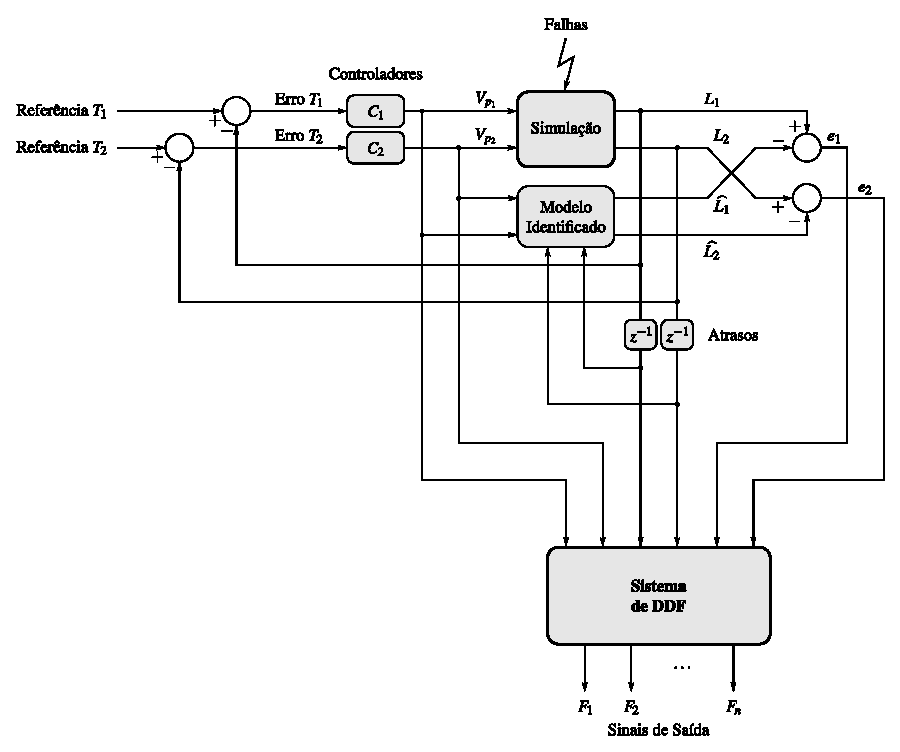
\includegraphics[width=0.9\textwidth]{imgs/sistema/eps/composicao}
    \caption{Composição do sistema proposto.}
    \label{fig:composicao}
\end{figure}

Acoplar tal sistema à um ambiente de monitoramento e supervisão, ou ainda
associá-lo à técnicas de controle tolerante à falhas, consiste simplesmente em
processar as informações disponíveis na interface de saída do módulo de DDF.
Contudo, isso não faz parte do escopo deste trabalho.
